\subsection{Modelos de S\'eries Temporais Univariados}\label{subsec:arima}

A previsão de séries temporais é um desafio complexo, sem uma resposta fácil. Existem inúmeros modelos estatísticos que afirmam superar uns aos outros, mas nunca está claro qual modelo é o melhor.

Dito isto, os modelos baseados em ARMA são frequentemente uma boa opção para iniciar. Eles podem alcançar pontuações decentes na maioria dos problemas de séries temporais e são adequados como modelos de referência em tais problemas.

Quanto ao modelo ARIMA, ele é dividido em três componentes: AR (Auto-Regressão), I (Integração) e MA (Média Móvel). O componente AR leva em consideração os valores anteriores da série temporal, o componente I trata das diferenças entre os valores observados para tornar a série estacionária, e o componente MA considera os erros residuais do modelo. Esses componentes combinados ajudam a capturar os padrões e tendências presentes na série temporal.

\subsubsection{Componente Autorregressivo}

O componente autoregressivo do modelo ARIMA é representado por AR(p), em que o parâmetro p determina o número de séries temporais defasadas utilizadas.

A equação do modelo AR(p) é expressa da seguinte forma:

\begin{eqnarray}
	Y_t&=&c+\sum_{n=1}^{p} \alpha_n Y_{t-n} + \varepsilon_t\label{AR}
\end{eqnarray}

A partir dos dados, é possível obter uma previsão utilizando o modelo AR(7).

\begin{figure}[H]
	\centering
	\caption{Comparação dos modelos AR e ARX}
	\begin{subfigure}{1\textwidth}
		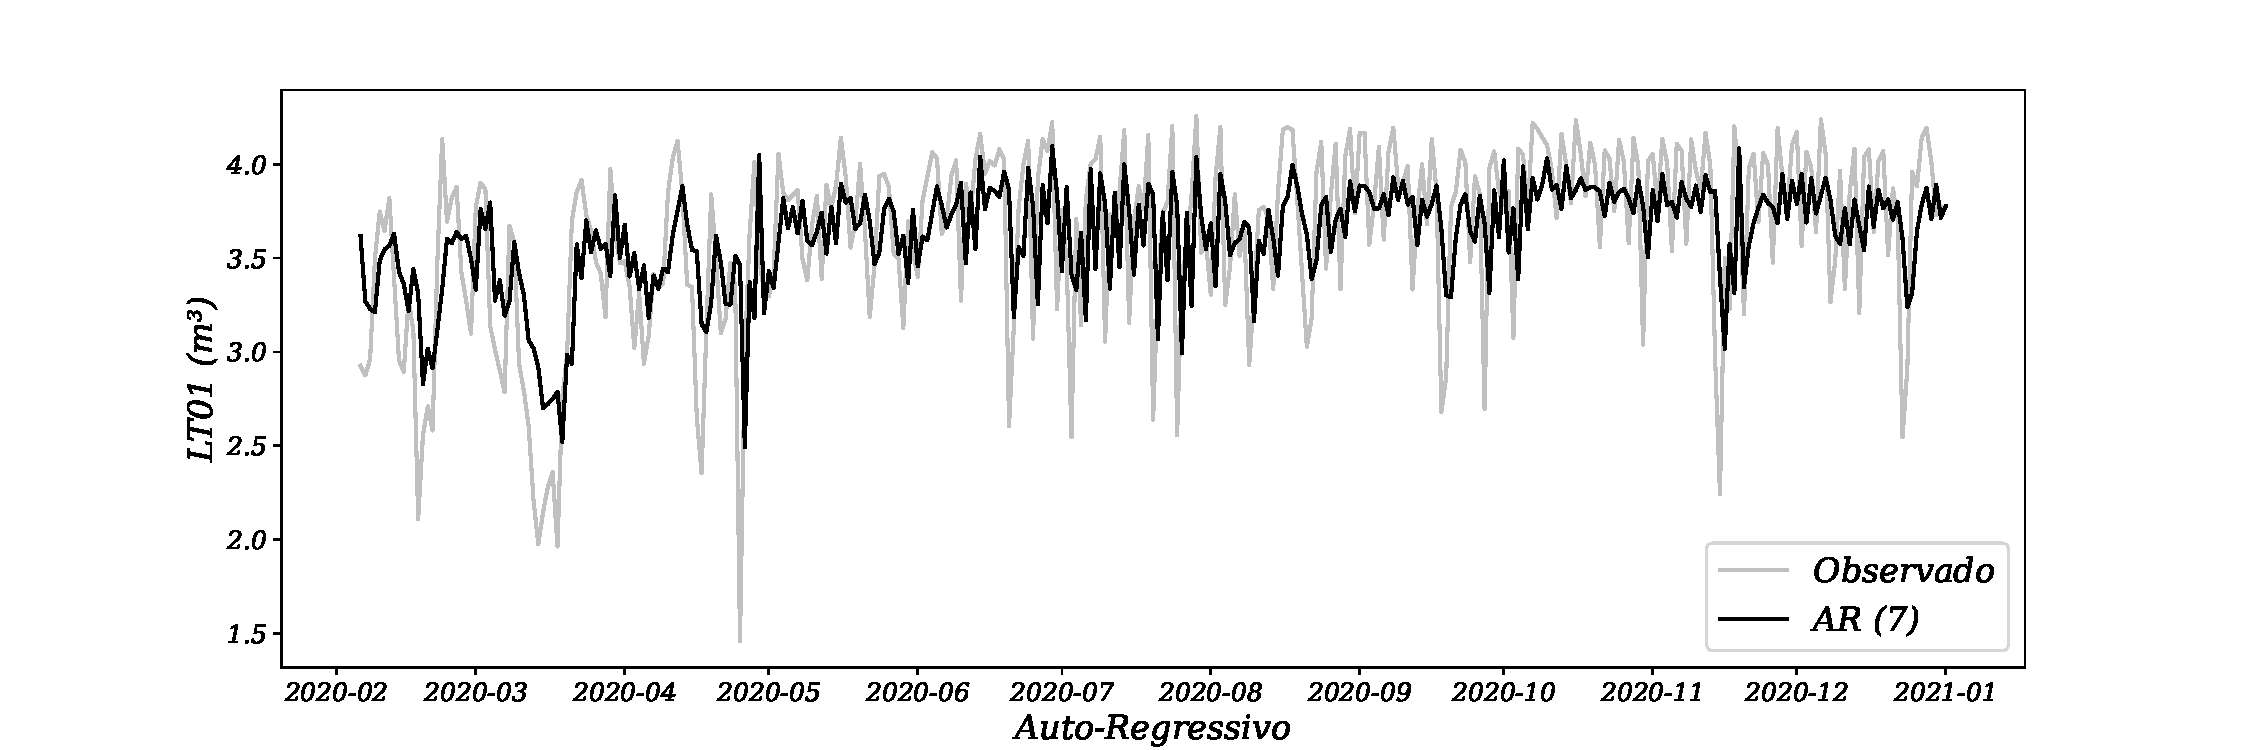
\includegraphics[width=\linewidth]{Modelos/Figuras/AR}
		\caption{Modelo AR(7)}
		\label{fig:1-ar}	
	\end{subfigure}
	
	\begin{subfigure}{1\textwidth}
		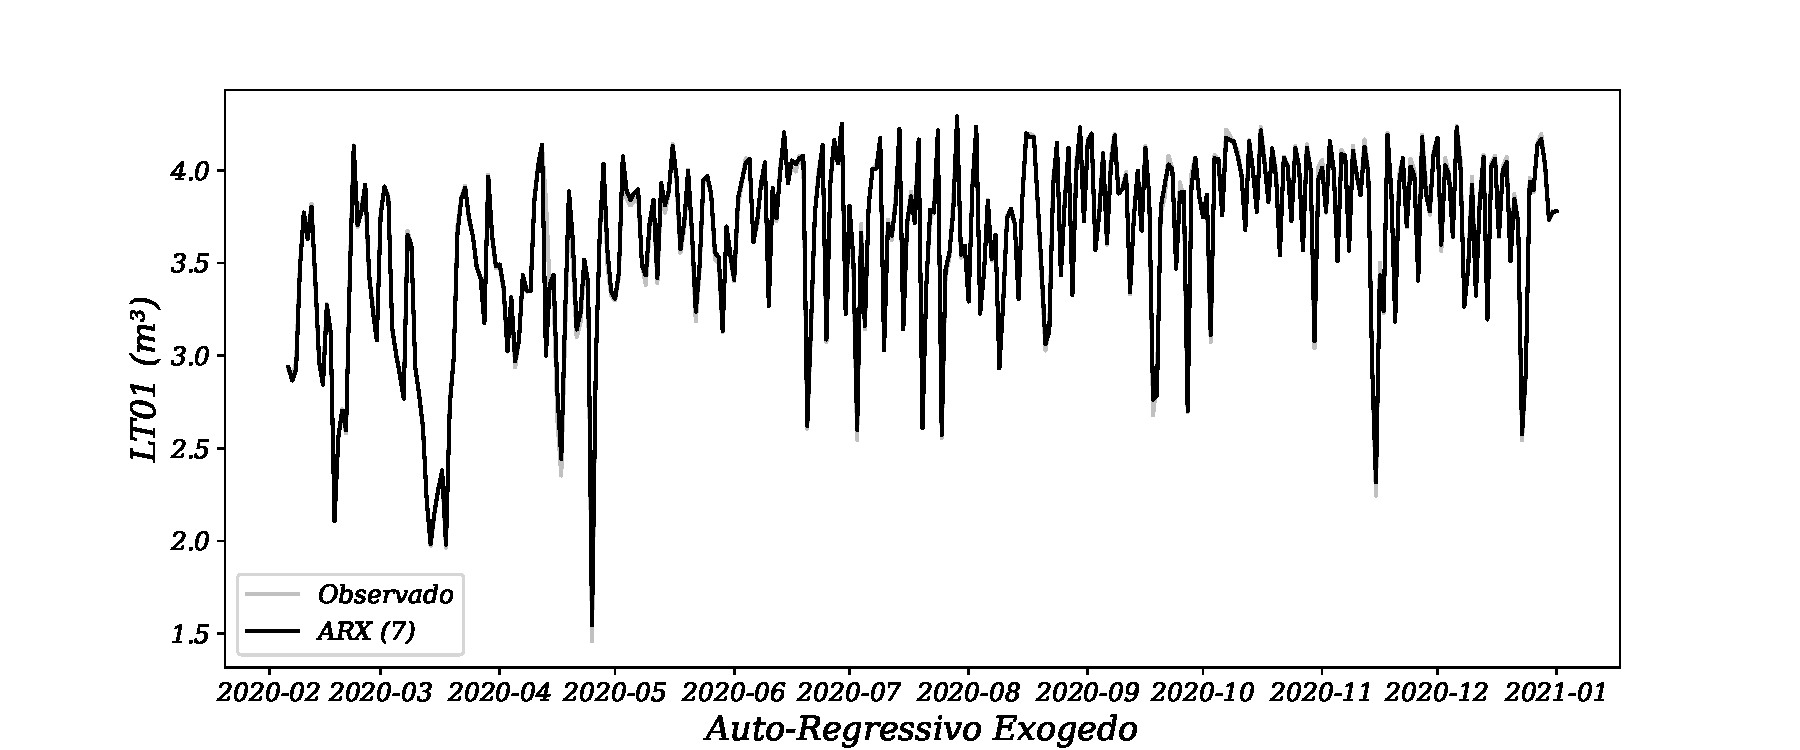
\includegraphics[width=\linewidth]{Modelos/Figuras/ARX}
		\caption{ARX (7)}
		\label{fig:1-arx}	
	\end{subfigure}
	
	\fonte{Elaboração própria a partir de dados da SANEPAR (2018 a 2020)}
\end{figure}



Na equação \eqref{AR}, o termo $\varepsilon_t$ representa o ruído branco. Essa equação pode ser entendida como uma regressão múltipla, em que os valores defasados de $y_t$ são utilizados como preditores. Esse modelo é conhecido como modelo autorregressivo de ordem $p$, ou AR(p).

A Figura \ref{fig:1-ar} tem como objetivo apresentar uma previsão de um passo à frente (um dia). Nos apêndices \ref{sec:ararxma24}, pode-se observar uma comparação entre os modelos AR, MA e ARX.

O modelo ARX é uma extensão do modelo AR, que incorpora variáveis exógenas nos dados para melhorar as previsões futuras. Esse modelo também é multivariado, como mostrado na subseção \ref{subsec:mult}, e foi incluído aqui para fins de comparação com o modelo AR simples, considerando a presença de variáveis exógenas.

Embora o modelo AR possa ser visualmente adequado para a previsão que está sendo feita, é importante destacar que, por ser um modelo autorregressivo, ele realiza previsões lineares e não captura padrões não lineares presentes nos dados. Para uma análise mais abrangente da série temporal, é necessário considerar exemplos de casos gerais.

\subsubsection{AR(0): Ru\'ido branco}

Se o parâmetro $p$ for definido como zero (AR($0$)), significa que não há termos autorregressivos no modelo. Nesse caso, a série temporal se comporta como um ruído branco. Cada ponto de dados é amostrado de uma distribuição com média zero e variância igual a sigma-quadrado. Isso resulta em uma sequência de números aleatórios que não exibem nenhum padrão ou correlação.

Essa propriedade do ruído branco pode ser útil em análises estatísticas, pois serve como uma hipótese nula. Ao comparar diferentes modelos ou testar a presença de padrões em uma série temporal, podemos usar o ruído branco como referência para avaliar se os resultados observados são estatisticamente significativos ou apenas resultado do acaso. Isso nos ajuda a evitar a detecção de padrões falsos positivos e garante a confiabilidade das análises realizadas.

\subsubsection{AR(1): Caminhadas aleat\'orias e Oscila\c c\~oes}

Com o parâmetro $p$ definido como $1$, o modelo AR leva em consideração o valor anterior da série temporal multiplicado por um coeficiente e, em seguida, adiciona ruído branco. Quando o coeficiente é igual a $0$, temos apenas ruído branco, resultando em uma série de tempo completamente aleatória, sem padrões previsíveis.

Quando o coeficiente é igual a $1$, temos uma caminhada aleatória, onde cada valor da série é obtido somando-se o valor anterior a um termo de ruído branco. Nesse caso, os valores da série apresentam uma tendência linear, aumentando ou diminuindo ao longo do tempo sem retornar à média.

Se o coeficiente estiver na faixa $0 < \alpha < 1$, temos o fenômeno de reversão média. Isso significa que os valores da série tendem a oscilar em torno de uma média central e a regressar em direção a ela após se afastarem. Esse padrão indica uma tendência de retorno à média ao longo do tempo.

Os diferentes comportamentos da série temporal, determinados pelo coeficiente no modelo AR, têm implicações importantes na análise e previsão de dados. A compreensão desses padrões é fundamental para escolher o modelo adequado e interpretar corretamente os resultados obtidos.

\subsubsection{AR(p): Termos de ordem superior}

Aumentar ainda mais o parâmetro $p$ no modelo AR significa considerar um número crescente de medições de tempo anteriores, cada uma multiplicada pelo seu próprio coeficiente. Isso permite levar em conta uma memória mais longa da série temporal e capturar padrões de dependência mais complexos ao longo do tempo.

No entanto, é importante ter em mente que aumentar excessivamente o valor de $p$ pode levar a problemas de \textit{overfitting}, onde o modelo se ajusta muito bem aos dados de treinamento, mas tem um desempenho ruim na previsão de novos dados. Portanto, é necessário encontrar um equilíbrio entre a complexidade do modelo e sua capacidade de generalização.

Além disso, é comum combinar o modelo AR com o modelo de média móvel (MA) para formar o modelo ARMA. O modelo MA considera os erros passados, ou seja, as diferenças entre os valores reais e as previsões anteriores, ajustadas por coeficientes. A combinação dos componentes AR e MA permite capturar tanto a dependência autorregressiva quanto a dependência na média móvel, proporcionando uma modelagem mais abrangente da série temporal.

Em suma, aumentar o parâmetro $p$ no modelo AR pode melhorar a capacidade do modelo de capturar padrões complexos da série temporal, mas é necessário ter cuidado para evitar \textit{overfitting}. A combinação com o modelo MA pode fornecer uma modelagem mais completa dos dados. A escolha adequada dos parâmetros depende da análise cuidadosa dos padrões presentes na série temporal e do equilíbrio entre a complexidade do modelo e sua capacidade de generalização.

\subsubsection{M\'edia M\'ovel}\label{subsubsec:ma}
No modelo de média móvel (MA), o componente não é uma média móvel simples, mas sim uma combinação de termos de erro de previsão defasados. O parâmetro $q$ no modelo MA representa o número de termos de erro de previsão que são levados em consideração na previsão.

De acordo com \citeonline{signal} este componente não é uma média de rolamento, mas sim os atrasos no ruído branco.

Em um modelo MA(1), por exemplo, a previsão é composta por um termo constante, o produto do termo de erro de previsão anterior por um multiplicador, e o termo de erro de previsão atual. Essa abordagem baseia-se em princípios estatísticos e de probabilidade, ajustando a previsão com base em termos anteriores de erro de previsão.

O modelo MA é uma alternativa ao modelo AR e é usado para capturar padrões de dependência na média móvel, ou seja, a influência de erros passados na previsão atual. Ao combinar o modelo AR e o modelo MA, como no modelo ARMA, é possível obter uma modelagem mais abrangente que considera tanto a dependência autorregressiva quanto a dependência na média móvel.

Portanto, o modelo MA leva em conta os termos de erro de previsão defasados para ajustar a previsão atual, permitindo considerar a probabilidade e estatística na modelagem da série temporal.


\begin{eqnarray}
	y_t=c+\varepsilon_t+\theta_1 \varepsilon_{t-1}+\theta_2 \varepsilon_{t-2}+\cdots+\theta_q \varepsilon_{t-q}\label{eq:ma}
\end{eqnarray}

Na equação \eqref{eq:ma}, em que $\varepsilon_t$ representa o ruído branco, esse modelo é conhecido como um modelo de média móvel $MA(q)$, em que $q$ é a ordem da média móvel. É importante ressaltar que não observamos diretamente os valores de $\varepsilon_t$, portanto, essa modelagem não se trata de uma regressão no sentido convencional.

Diferentemente de uma regressão comum em que temos variáveis explicativas observadas, no modelo $MA(q)$, estamos usando os termos de ruído branco defasados para estimar e prever os valores da série temporal. O objetivo é capturar a dependência dos termos de erro passados na previsão atual.

Esse modelo é útil para modelar séries temporais em que a média móvel tem um impacto significativo nas observações. Ao ajustar a série temporal com base nos termos de ruído branco defasados, podemos obter uma estimativa mais precisa dos valores futuros.

Embora o modelo $MA(q)$ seja diferente de uma regressão tradicional, ele é uma ferramenta estatística poderosa para modelar e prever séries temporais, levando em consideração a dependência entre os termos de erro passados.

\begin{figure}[H]
	\centering
	\caption{Modelo MA(7) }
	\label{fig:1-ma}
	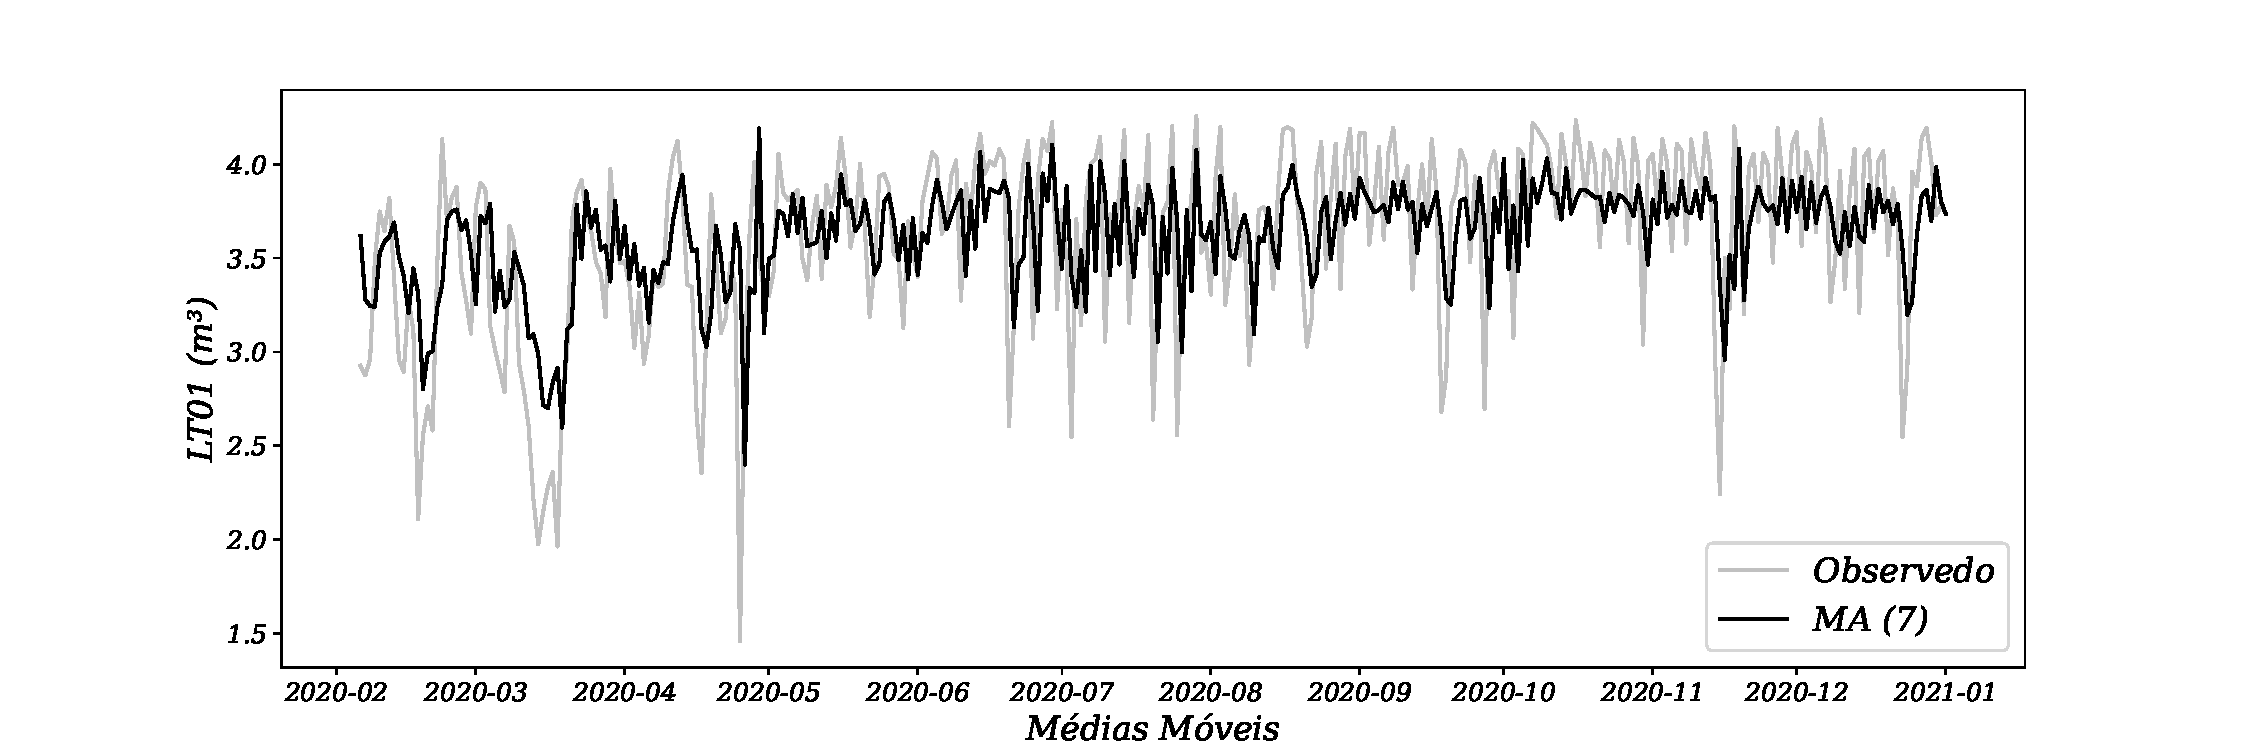
\includegraphics[width=1\linewidth]{Modelos/Figuras/MA}
	
	\fonte{Elaboração própria a partir de dados da SANEPAR (2018 a 2020)}
\end{figure}

O modelo MA, quando comparado com o modelo AR de mesma ordem, facilita a previsão. Conforme ilustrado na Figura \ref{fig:1-ma}, a previsão gráfica se assemelha ao modelo apresentado na Figura \ref{fig:1-ar}, embora não seja comparável ao modelo exibido na Figura \ref{fig:1-arx}. É importante notar que esse modelo aparenta prever com precisão o período de tempo que foi considerado.

\subsubsection{Modelos ARMA e ARIMA}\label{subsubsec:arma}
A arquitetura ARMA é uma combinação dos modelos AR  e MA, onde o modelo AR é adicionado ao modelo MA.

No modelo ARMA, é adicionada uma constante à soma dos termos autorregressivos multiplicados pelos seus coeficientes, juntamente com a soma dos termos de média móvel multiplicados pelos seus coeficientes, além do ruído branco. Essa estrutura é amplamente utilizada em diversos modelos de previsão em diferentes áreas.

\begin{figure}[H]
	\centering
	\caption{ARMA (7,7)}
	\label{fig:1-arma}
	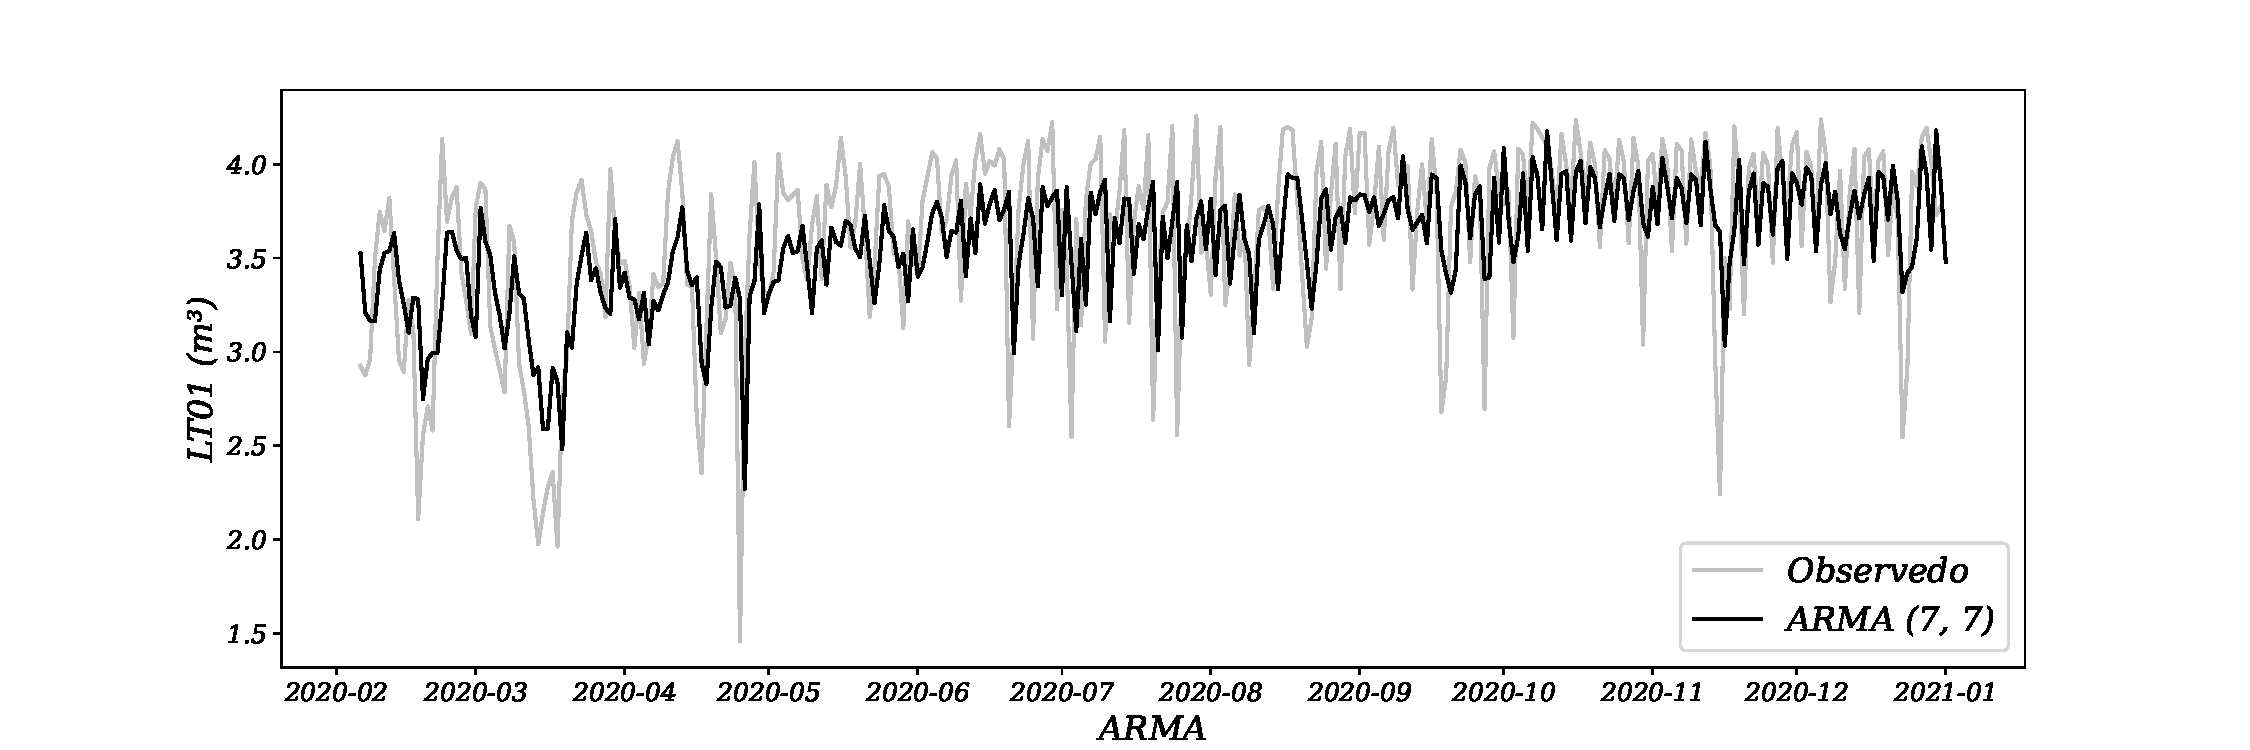
\includegraphics[width=1\linewidth]{Modelos/Figuras/ARMA}
	
	\fonte{Elaboração própria a partir de dados da SANEPAR (2018 a 2020)}
\end{figure}

A Figura \ref{fig:1-arma} ilustra a combinação dos modelos AR e MA em um modelo ARMA. Essa abordagem pode levar a uma redução significativa no erro de previsão, como observado nos apêndices \ref{sec:comtb24} e \ref{sec:comtb18}, onde são apresentadas comparações com um maior número de passos de previsão.

\subsubsection{ARIMA}

\begin{eqnarray}
	Y_t = \beta_2 + \omega_1\varepsilon_{t-1} + \omega_2 \varepsilon_{t-2} +\ldots+ \omega_q \varepsilon_{t-q} + \varepsilon_t \label{arima}
\end{eqnarray}

Na equação \eqref{arima}, a variável $Y_t$ representa a série temporal que foi diferenciada (possivelmente mais de uma vez). Os "preditores" no lado direito da equação incluem os valores defasados de $Y_t$ e os erros defasados. Esse tipo de modelo é conhecido como ARIMA ($p, d, q$).

O modelo ARIMA é uma extensão do modelo ARMA que incorpora uma etapa adicional de pré-processamento chamada de diferenciação. Essa etapa é representada pela notação \textbf{I(d)}, em que \textbf{d} denota a ordem de diferenciação, ou seja, o número de transformações necessárias para tornar a série temporal estacionária. Portanto, um modelo ARIMA é simplesmente um modelo ARMA aplicado à série temporal diferenciada. Isso permite lidar com séries temporais que possuem tendências ou padrões não estacionários.

\begin{figure}[H]
	\centering
	\caption{ARIMA (7,1,7)}
	\label{fig:1-arima}
	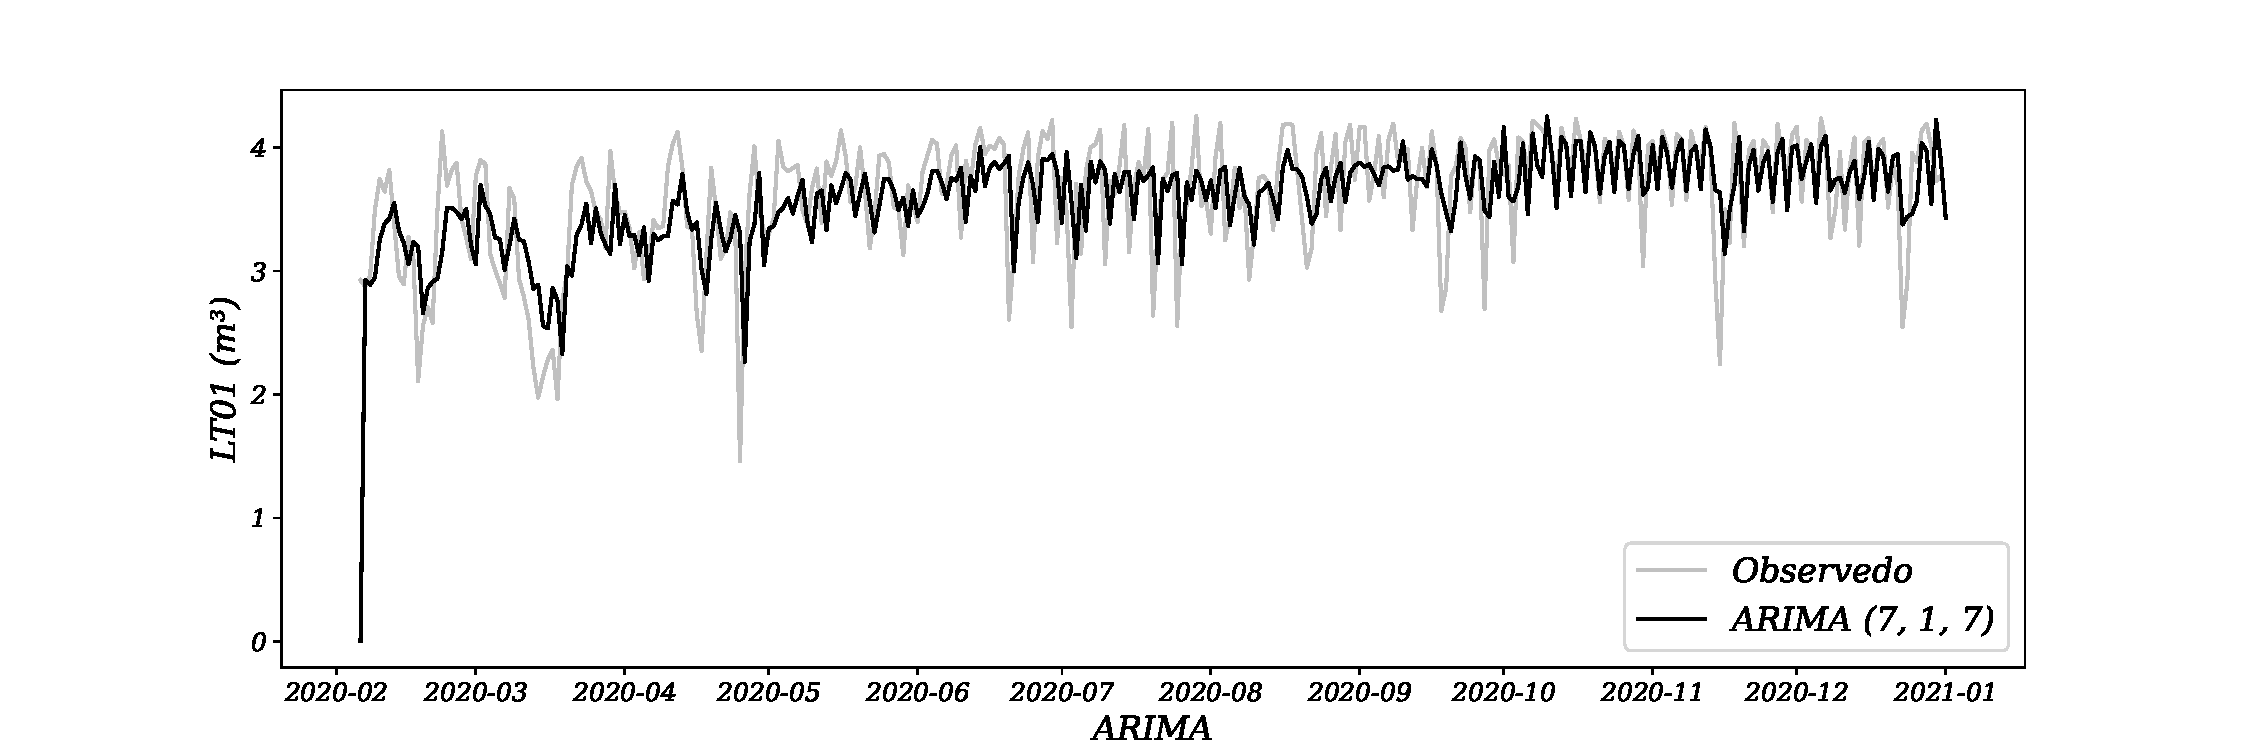
\includegraphics[width=1\linewidth]{Modelos/Figuras/ARIMA}
	
	Fonte: Elaboração própria a partir de dados da SANEPAR (2018 a 2020)
\end{figure}

Ao analisar a Figura \ref{fig:1-arima}, não se nota uma diferença visual significativa em relação aos outros métodos apresentados anteriormente. O método ARX ainda parece ser superior aos demais com base na análise visual.

Embora os modelos ARIMA sejam eficazes, incorporar variáveis sazonais e exógenas ao modelo pode potencializar sua capacidade de previsão. No entanto, é importante destacar que o modelo ARIMA pressupõe que a série temporal seja estacionária. Quando lidamos com séries temporais não estacionárias, é necessário recorrer a outros modelos para a análise e previsão adequadas.

\subsubsection{SARIMA}

\begin{eqnarray}
	Y_t&=&c+\sum_{n=1}^p \alpha_n y_{t-n}+\sum_{n=1}^q \theta_n \epsilon_{t-n}+\sum_{n=1}^P \phi_n y_{t-s n}+\sum_{n=1}^Q \eta_n \epsilon_{t-s n}+\epsilon_t \label{sarima}
\end{eqnarray}

O modelo proposto é uma extensão do modelo ARIMA, com a adição de componentes autorregressivos e de média móvel sazonal. Esses componentes extras são ajustados levando em consideração os padrões sazonais presentes nos dados, utilizando atrasos correspondentes à frequência sazonal (por exemplo, 12 para dados mensais). Essa abordagem permite capturar e modelar de forma mais precisa as variações sazonais e melhorar a qualidade das previsões em séries temporais com esse comportamento cíclico.

\begin{figure}[H]
	\centering
	\caption{SARIMA $(7,1,7) (2,1,1)_{12}$}
	\label{fig:1-sarima}
	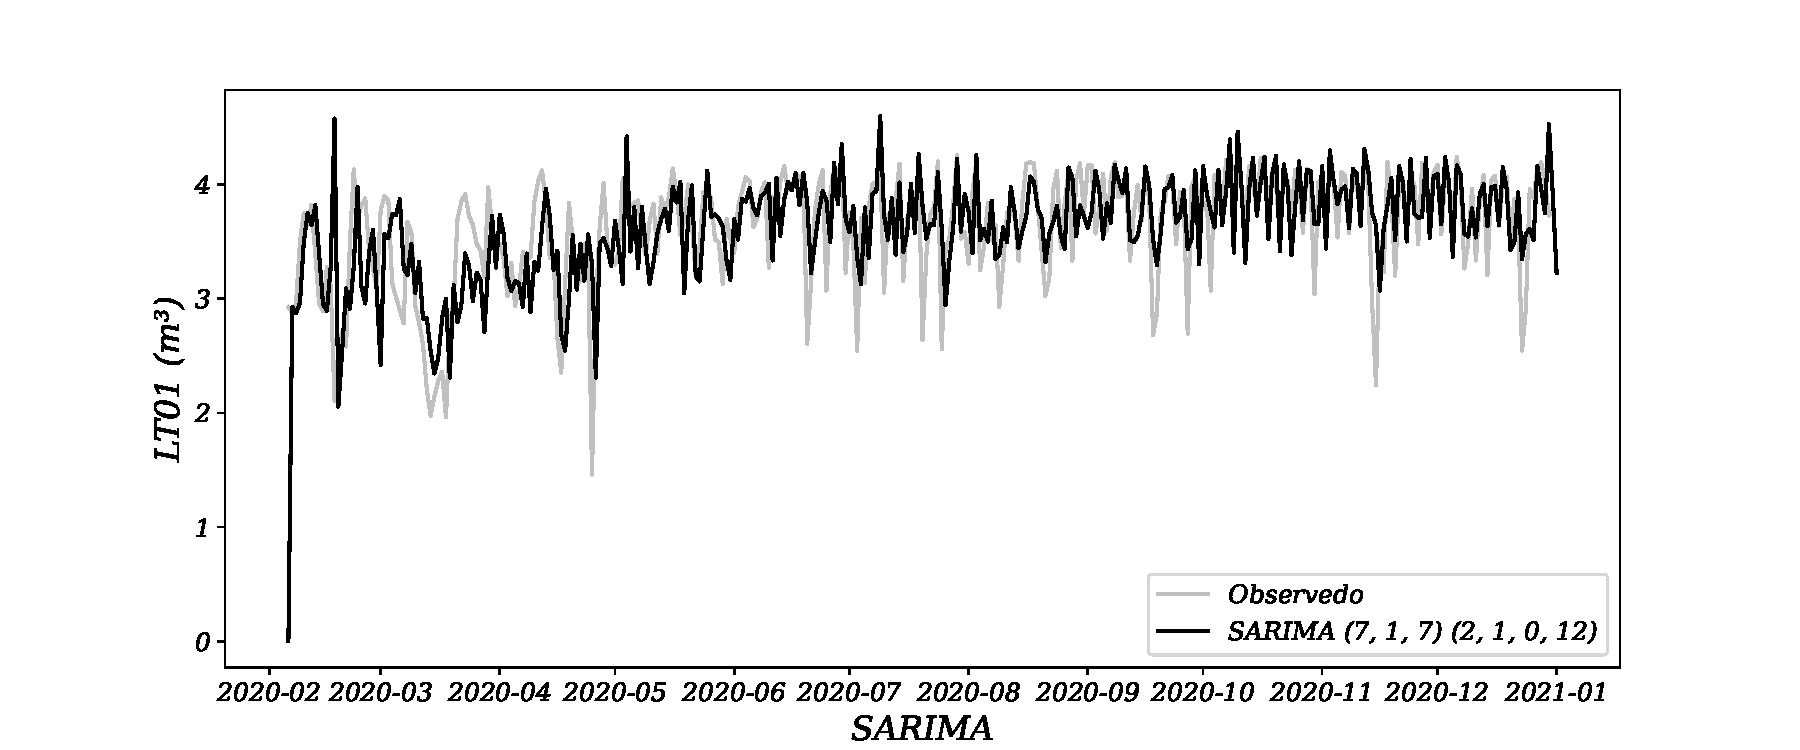
\includegraphics[width=1\linewidth]{Modelos/Figuras/SARIMA}
	
	\fonte{Elaboração própria a partir de dados da SANEPAR (2018 a 2020)}
\end{figure}

Na Figura \ref{fig:1-sarima}, é possível observar que a previsão em vermelho está mais próxima dos valores observados em preto, mostrando que a inclusão do componente de sazonalidade melhora a qualidade da previsão. Os modelos SARIMA são capazes de lidar com dados que apresentam padrões sazonais, permitindo a diferenciação dos dados em termos de componentes sazonais e não sazonais. Uma abordagem útil para determinar os melhores parâmetros do modelo é utilizar uma estrutura de pesquisa automatizada de parâmetros, como o pmdarima, que auxilia na identificação dos parâmetros ideais para o modelo SARIMA. Isso pode contribuir para uma melhor compreensão e ajuste do modelo aos dados observados.

\subsection{Modelos de S\'erie Temporal Multivariada}\label{subsec:mult}

Os Modelos de Série Temporal Multivariada são uma abordagem estatística utilizada para analisar e prever dados que possuem múltiplas variáveis dependentes ao longo do tempo. Nesse tipo de modelo, considera-se a interdependência entre as diferentes séries temporais, permitindo a análise conjunta e a identificação de padrões e relações entre as variáveis. Esses modelos são aplicados em diversas áreas, como economia, finanças, meteorologia e análise de dados, proporcionando insights valiosos para a compreensão e previsão de fenômenos complexos ao longo do tempo.

\subsubsection{ARIMAX e SARIMAX}

\begin{eqnarray}
	d_t=c+\sum_{n=1}^p \alpha_n d_{t-n}+\sum_{n=1}^q \theta_n \epsilon_{t-n}+\sum_{n=1}^r \beta_n x_{n_t}+\sum_{n=1}^P \phi_n d_{t-s n}+\sum_{n=1}^Q \eta_n \epsilon_{t-s n}+\epsilon_t \label{eq:sarmax}
\end{eqnarray}

Em \eqref{eq:sarmax}, o modelo SARIMAX é apresentado. Nesse modelo, são consideradas variáveis exógenas, ou seja, são utilizados dados externos para a realização das previsões. É importante ressaltar que mesmo que essas variáveis exógenas sejam indiretamente modeladas no histórico de previsões do modelo, ao incluí-las diretamente, o modelo será capaz de responder de forma mais ágil aos efeitos dessas variáveis. Isso significa que a incorporação de informações externas possibilita uma resposta mais rápida e precisa do modelo em relação aos fatores externos, resultando em previsões mais atualizadas e acuradas.

\begin{figure}[htpb!]
	\centering
	\caption{Comparação entre ARIMAX e SARIMAX}
	\begin{subfigure}{1\textwidth}
		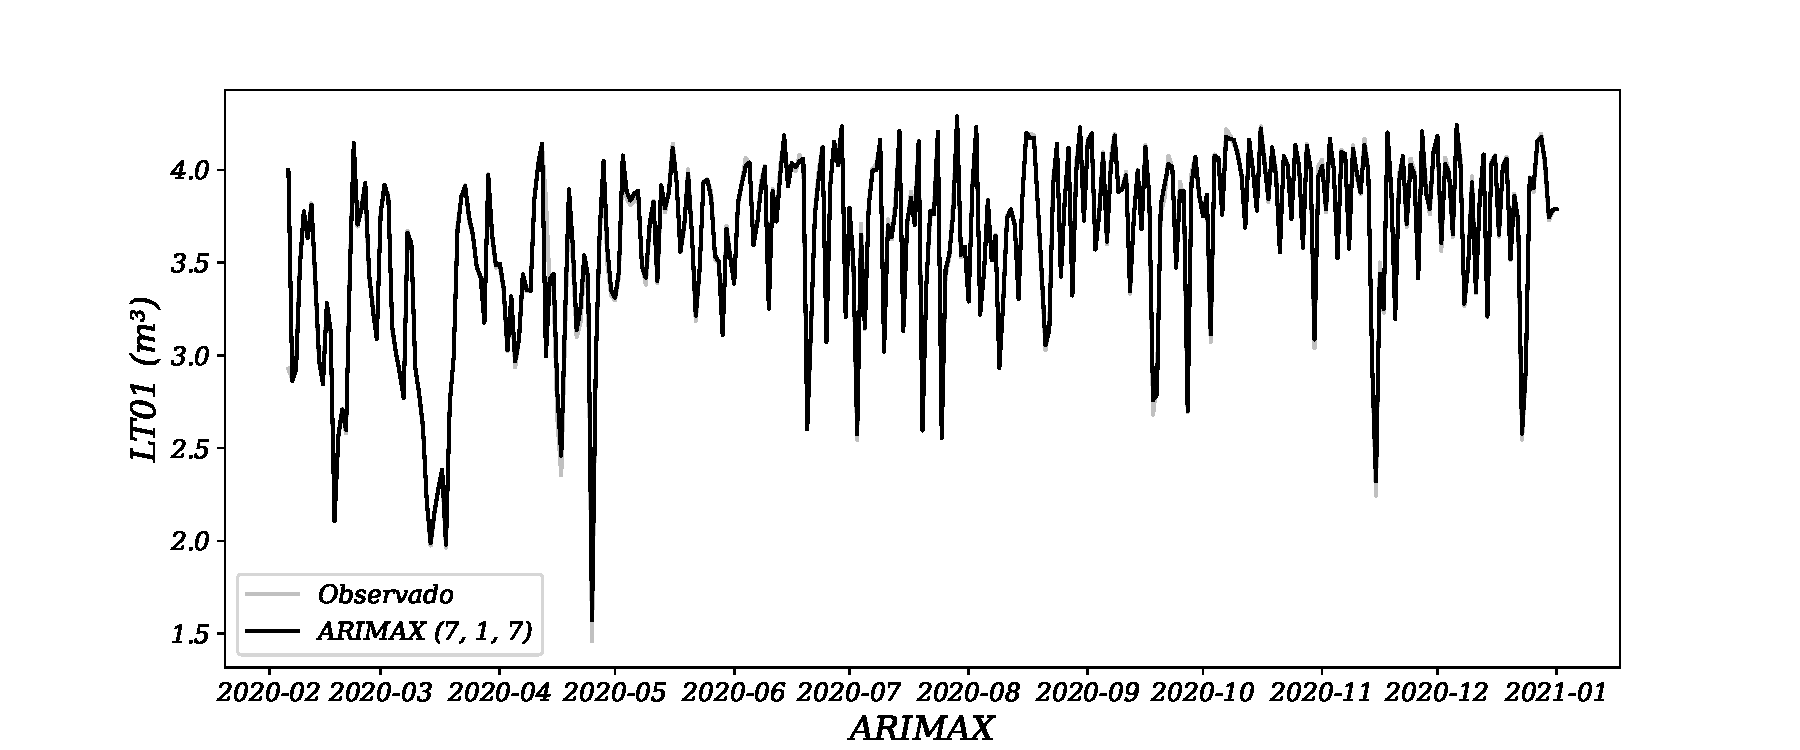
\includegraphics[width=\linewidth]{Modelos/Figuras/ARIMAX}
		\caption{ARIMAX $(7,1,7)$}
		\label{fig:1-arimax}
	\end{subfigure}
	\hfill
	
	\begin{subfigure}{1\textwidth}
		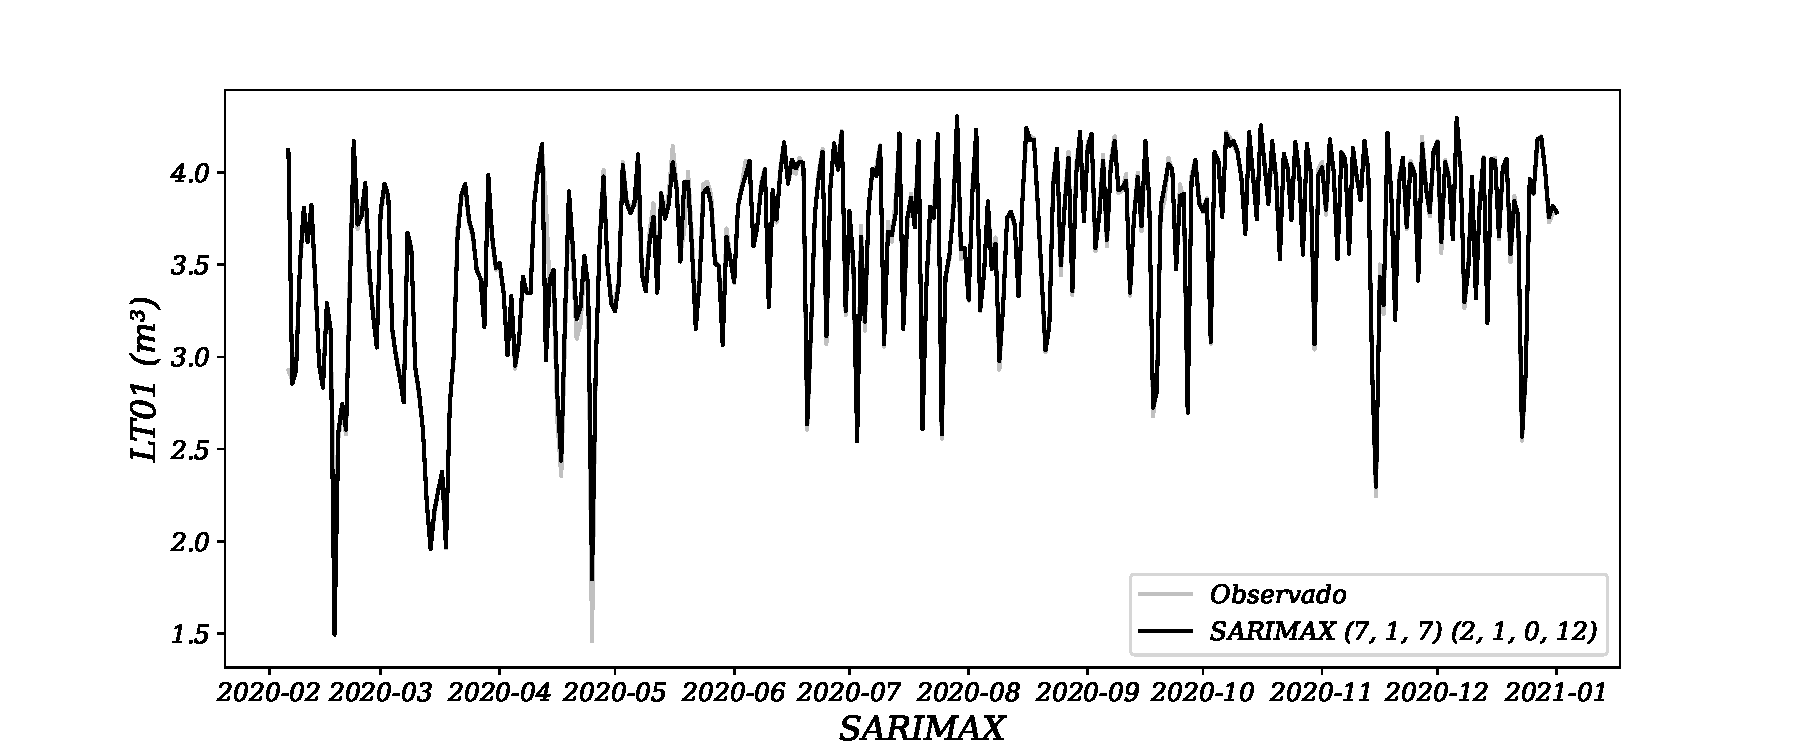
\includegraphics[width=\linewidth]{Modelos/Figuras/SARIMAX}
		\caption{SARIMAX $(7,1,7) (2,1,1)_{12}$}
		\label{fig:1-sarimax}	
	\end{subfigure}

		
	\fonte{Elaboração própria a partir de dados da SANEPAR (2018 a 2020)}
\end{figure}


Entre os modelos com variáveis exógenas, como mostrado nas Figuras \ref{fig:1-arimax} e \ref{fig:1-sarimax}, observa-se uma melhora significativa na qualidade das previsões em comparação com os modelos que não incluem variáveis exógenas. A adição dessas variáveis externas permite capturar melhor as influências e os padrões presentes nos dados, resultando em previsões mais completas e precisas. Essa inclusão de informações adicionais contribui para uma compreensão mais abrangente do comportamento da série temporal e possibilita uma melhor adaptação do modelo aos padrões observados.
